\documentclass[11pt]{article}

\usepackage[a4paper,margin=1in]{geometry}
\usepackage[T1]{fontenc}
\usepackage[utf8]{inputenc}
\usepackage{lmodern}
\usepackage{amsmath,amssymb,mathtools}
\usepackage{booktabs}
\usepackage{graphicx}
\usepackage{xcolor}
\usepackage{hyperref}

\hypersetup{
  colorlinks=true,
  linkcolor=blue!60!black,
  citecolor=blue!60!black,
  urlcolor=blue!60!black
}

\newcommand{\ii}{\mathrm{i}}
\newcommand{\Ds}{D_s}
\newcommand{\Dsone}{D_{s1}}
\newcommand{\Bs}{B_s}
\newcommand{\Bsone}{B_{s1}}
\newcommand{\GeV}{\mathrm{GeV}}
\newcommand{\MeV}{\mathrm{MeV}}
\newcommand{\keV}{\mathrm{keV}}
\newcommand{\qqbar}{\langle\bar q q\rangle}
\newcommand{\ssbar}{\langle\bar s s\rangle}

\title{Radiative Transitions of Strange Heavy Axial Mesons in Light-Cone QCD Sum Rules}
\author{S. Bilmis et al.}
\date{\today}

\begin{document}
\maketitle

\begin{abstract}
We study the radiative transitions
$\Dsone(2460)\to\Ds\gamma$, $\Dsone(2536)\to\Ds\gamma$, and
$\Bsone(5830)\to\Bs\gamma$ with light-cone QCD sum rules.  The calculation
includes hard photon emission from both quark lines, two-particle photon
distribution amplitudes, and three-particle photon distribution-amplitude
corrections from the background-gluon term in the quark propagator.  The
strange-quark mass is retained explicitly.  We compare a legacy
magnetic-susceptibility photon input with a recent lattice normalization of the
leading-twist photon distribution amplitude.  For the charm-strange channels we
include a physical-current residue normalization calibrated by local QCD sum
rules, while for the bottom-strange channel we use a Pullin--Zwicky
decay-constant scenario.  The preferred lattice-normalized results give a
moderate width for $\Dsone(2460)\to\Ds\gamma$, a strongly cancellation
suppressed $\Dsone(2536)\to\Ds\gamma$ width, and a sub-keV median prediction
for $\Bsone(5830)\to\Bs\gamma$.
\end{abstract}

\section{Introduction}

Radiative decays of positive-parity strange heavy mesons provide a sensitive
probe of their spin structure, electromagnetic couplings, and proximity to
open-flavor thresholds.  The charm-strange states $\Dsone(2460)$ and
$\Dsone(2536)$ have long been discussed in this context, and
$\Dsone(2460)\to\Ds\gamma$ has an experimentally measured branching fraction
\cite{BaBar2006}.  The high state $\Dsone(2536)$ has a measured total width
\cite{BaBar2011}, but its radiative decay to $\Ds\gamma$ is expected to be
small.  The bottom-strange state $\Bsone(5830)$ is observed spectroscopically
\cite{CMS2018}, while its radiative decay remains a target for future searches.

The purpose of this work is to update the light-cone sum-rule analysis of
these radiative channels with a transparent separation of hard photon emission,
two-particle photon distribution amplitudes (DAs), and three-particle photon
DAs.  We keep explicit $m_s$ effects and track the normalization associated
with the two physical axial currents.  We also compare the older
magnetic-susceptibility input for the photon DA \cite{Ball:2002ps,Rohrwild2007}
with the recent lattice normalization of the leading-twist photon DA
\cite{Bacchio2024}.

\section{Conventions and Hadronic Representation}

We use the mostly-minus metric, $\epsilon^{0123}=+1$, and the momentum
assignment
\begin{equation}
  P=p+q,
\end{equation}
where $P$ is the initial axial-meson momentum, $p$ is the final pseudoscalar
momentum, and $q$ is the real-photon momentum.  The pseudoscalar interpolating
current is
\begin{equation}
  J_5(x)=\bar s(x)\,\ii\gamma_5\,Q(x),
\end{equation}
with $Q=c$ or $b$.  For the axial channel we use the two basis currents
\begin{align}
  J^{A}_{\mu}(x) &= \bar s(x)\gamma_\mu\gamma_5 Q(x),\\
  J^{B}_{\mu}(x) &=
  \frac{\ii}{m_Q+m_s}\bar s(x)\sigma_{\mu\alpha}P^\alpha\gamma_5 Q(x).
\end{align}
The tensor current therefore carries the initial-state momentum $P^\alpha$.
The physical-current combinations are taken as
\begin{align}
  J_{1\mu} &= \sin\theta\,J^A_\mu+\cos\theta\,J^B_\mu,\\
  J_{2\mu} &= \cos\theta\,J^A_\mu-\sin\theta\,J^B_\mu,
\end{align}
with central $\theta=35.3^\circ$ and a scan over
$25^\circ\leq\theta\leq45^\circ$.

The transition amplitude is parametrized by an E1 coupling $G$,
\begin{equation}
  \langle P(p)\gamma(q,\varepsilon)|A(P,\eta)\rangle
  =
  e\,G\left[(\eta\cdot\varepsilon^*)(p\cdot q)
  -(\eta\cdot q)(p\cdot\varepsilon^*)\right],
\end{equation}
so that
\begin{equation}
  \Gamma(A\to P\gamma)
  =
  \frac{\alpha_{\rm em}}{3}\,G^2\,|\vec q\,|^3,\qquad
  |\vec q\,|=\frac{m_A^2-m_P^2}{2m_A}.
  \label{eq:width}
\end{equation}

\section{Light-Cone Sum Rule}

The correlation function is
\begin{equation}
  \Pi_\mu(p,q)=\ii\int d^4x\,e^{\ii p\cdot x}
  \langle\gamma(q,\varepsilon)|
  T\{\bar s(x)\Gamma_\mu Q(x)\,\bar Q(0)\ii\gamma_5 s(0)\}
  |0\rangle ,
  \label{eq:corr}
\end{equation}
where $\Gamma_\mu$ denotes either the axial or tensor basis current.  We
project onto the transverse structure
\begin{equation}
  T_{\mu\nu}=(p\cdot q)g_{\mu\nu}-q_\mu p_\nu .
\end{equation}
The OPE includes:
\begin{itemize}
  \item hard photon emission from both the heavy and strange quark lines;
  \item two-particle photon DAs, including the leading-twist magnetic
  susceptibility or lattice-normalized transverse photon input;
  \item three-particle photon DAs generated by the background-gluon insertion
  in the quark propagator.
\end{itemize}
Ordinary vacuum-condensate terms are not inserted as separate corrections in
the base propagators of the three-point photon LCSR.  Condensate dependence
enters through photon matrix elements and photon-DA normalizations such as
$\chi_s\ssbar$.  This is distinct from a local two-point decay-constant sum
rule, where ordinary SVZ condensates do appear.

After Borel transformation and continuum subtraction, the basis-current
couplings are denoted by $G_A$ and $G_B$.  For the charm-strange physical
currents we use
\begin{align}
  G_{2460} &=
  \frac{\sin\theta\,f_A\,G_A+\cos\theta\,f_B\,G_B}{f_1},\\
  G_{2536} &=
  \frac{\cos\theta\,f_A\,G_A-\sin\theta\,f_B\,G_B}{f_2}.
  \label{eq:stage3}
\end{align}
The residue $f_1$ is calibrated from the local-QCDSR value
$f_{D_{s1}(2460)}=0.345\pm0.017~\GeV$ \cite{Wang2015}; the same two-point
overlap model predicts $f_2\simeq0.38~\GeV$.  For the bottom-strange channel
we quote a Pullin--Zwicky decay-constant scenario,
$f_{\Bsone}^{\rm PZ}=0.305\pm0.027~\GeV$ and
$f_{\Bsone}^{T,\rm PZ}=0.285\pm0.027~\GeV$ \cite{PullinZwicky2021}.  We do not
interpret the bottom effective mixed residue as an independently derived
local two-point $f_1$ or $f_2$.

\section{Numerical Inputs}

Table~\ref{tab:inputs} summarizes the main numerical inputs.  Masses, quark
masses, and electromagnetic normalization are taken from PDG summaries
\cite{PDG2024}; decay constants and lattice context are taken from FLAG and
related heavy-light sum-rule literature
\cite{FLAG2024,Colangelo2005,PullinZwicky2021,Wang2015}.  Photon DAs follow
Ball, Braun and Kivel \cite{Ball:2002ps}, the legacy magnetic susceptibility
comparison follows Rohrwild \cite{Rohrwild2007}, and the modern photon
normalization scenario uses Bacchio et al. \cite{Bacchio2024}.

\begin{table}[htbp]
  \centering
  \resizebox{\textwidth}{!}{%
  \begin{tabular}{llll}
    \toprule
    Quantity & Symbol & Value & Source/use\\
    \midrule
    quark masses & $m_c,m_b,m_s$ & $1.27(2),\,4.18(3),\,0.093(11)~\GeV$
      & PDG inputs, with explicit $m_s$ terms\\
    charm hadron masses & $M_{2460},M_{2536},m_{\Ds}$
      & $2.4595,\,2.53511,\,1.96835~\GeV$ & PDG\\
    bottom hadron masses & $M_{5830},m_{\Bs}$
      & $5.82870,\,5.36692~\GeV$ & PDG/CMS\\
    lower $\Bsone$ diagnostic mass & $M_{\Bsone}^{\rm low}$
      & $5.750(26)~\GeV$ & lattice-inspired diagnostic \cite{Lang2015}\\
    $\Ds$ and $\Bs$ decay constants & $f_{\Ds},f_{\Bs}$
      & $0.2499,\,0.2303~\GeV$ & FLAG/lattice context\\
    charm physical residues & $f_1,f_2$
      & $0.345(17),\,\simeq0.38~\GeV$ & Stage-3 normalization\\
    bottom PZ constants & $f_{\Bsone}^{\rm PZ},f_{\Bsone}^{T,\rm PZ}$
      & $0.305(27),\,0.285(27)~\GeV$ & PZ scenario\\
    legacy photon input & $\chi_s(1~\GeV)$
      & $+3.15(30)~\GeV^{-2}$ & comparison scenario\\
    lattice photon input & $f_{\gamma,s}^\perp(1~\GeV)$
      & $-55.1(1.9)~\MeV$ & preferred modern scenario\\
    \bottomrule
  \end{tabular}%
  }
  \caption{Main numerical inputs.  The complete bookkeeping tables are
  \texttt{inputs\_table.csv}, \texttt{outputs/paper\_input\_summary\_table.csv},
  and \texttt{outputs/input\_citation\_map.csv}.}
  \label{tab:inputs}
\end{table}

\section{Results}

The final form-factor and width predictions are shown in
Table~\ref{tab:main-results}.  The table quotes medians and 16--84 percentile
intervals.  Percentile intervals are preferred because several channels,
especially $\Dsone(2536)$ and $\Bsone(5830)$, are cancellation sensitive and
non-Gaussian near zero.

\begin{table}[htbp]
  \centering
  \resizebox{\textwidth}{!}{%
  \begin{tabular}{lllllcc}
    \toprule
    Sector & Decay & Photon input & Mixing & Normalization
      & $G~(\GeV^{-1})$ & $\Gamma~(\keV)$\\
    \midrule
    $D_s$ & $\Dsone(2460)\to\Ds\gamma$ & legacy $\chi_s$
      & $35.3^\circ$ & $f_1=0.344[0.329,0.363]$
      & $-0.424[-0.484,-0.360]$ & $37.7^{+11.5}_{-10.5}$\\
    $D_s$ & $\Dsone(2536)\to\Ds\gamma$ & legacy $\chi_s$
      & $35.3^\circ$ & $f_2=0.380[0.339,0.423]$
      & $+0.0118[+0.0014,+0.0233]$ & $0.045^{+0.124}_{-0.040}$\\
    $D_s$ & $\Dsone(2460)\to\Ds\gamma$ & lattice $f_{\gamma,s}^{\perp}$
      & $35.3^\circ$ & $f_1=0.345[0.330,0.364]$
      & $-0.277[-0.312,-0.243]$ & $16.1^{+4.4}_{-3.7}$\\
    $D_s$ & $\Dsone(2536)\to\Ds\gamma$ & lattice $f_{\gamma,s}^{\perp}$
      & $35.3^\circ$ & $f_2=0.379[0.338,0.423]$
      & $+0.0403[+0.0194,+0.0596]$ & $0.504^{+0.600}_{-0.377}$\\
    $B_s$ & $\Bsone(5830)\to\Bs\gamma$ & legacy $\chi_s$
      & $35.3^\circ$ & PZ constants, $f_{\rm eff}=0.391[0.354,0.428]$
      & $-0.0140[-0.0387,+0.0155]$ & $0.109^{+0.304}_{-0.101}$\\
    $B_s$ & $\Bsone(5830)\to\Bs\gamma$ & lattice $f_{\gamma,s}^{\perp}$
      & $35.3^\circ$ & PZ constants, $f_{\rm eff}=0.393[0.354,0.427]$
      & $+0.0356[+0.0029,+0.0694]$ & $0.272^{+0.752}_{-0.244}$\\
    $B_s$ & $\Bsone(5830)\to\Bs\gamma$ & legacy $\chi_s$
      & $25^\circ$--$45^\circ$ & PZ constants, $f_{\rm eff}=0.394[0.356,0.430]$
      & $-0.0126[-0.0527,+0.0364]$ & $0.249^{+0.570}_{-0.226}$\\
    $B_s$ & $\Bsone(5830)\to\Bs\gamma$ & lattice $f_{\gamma,s}^{\perp}$
      & $25^\circ$--$45^\circ$ & PZ constants, $f_{\rm eff}=0.387[0.348,0.423]$
      & $+0.0330[-0.0228,+0.0974]$ & $0.429^{+1.665}_{-0.401}$\\
    \bottomrule
  \end{tabular}%
  }
  \caption{Final form-factor and width summary.  The lattice photon input is
  our preferred modern normalization; the legacy susceptibility input is kept
  for comparison with older photon-DA analyses.}
  \label{tab:main-results}
\end{table}

\begin{figure}[htbp]
  \centering
  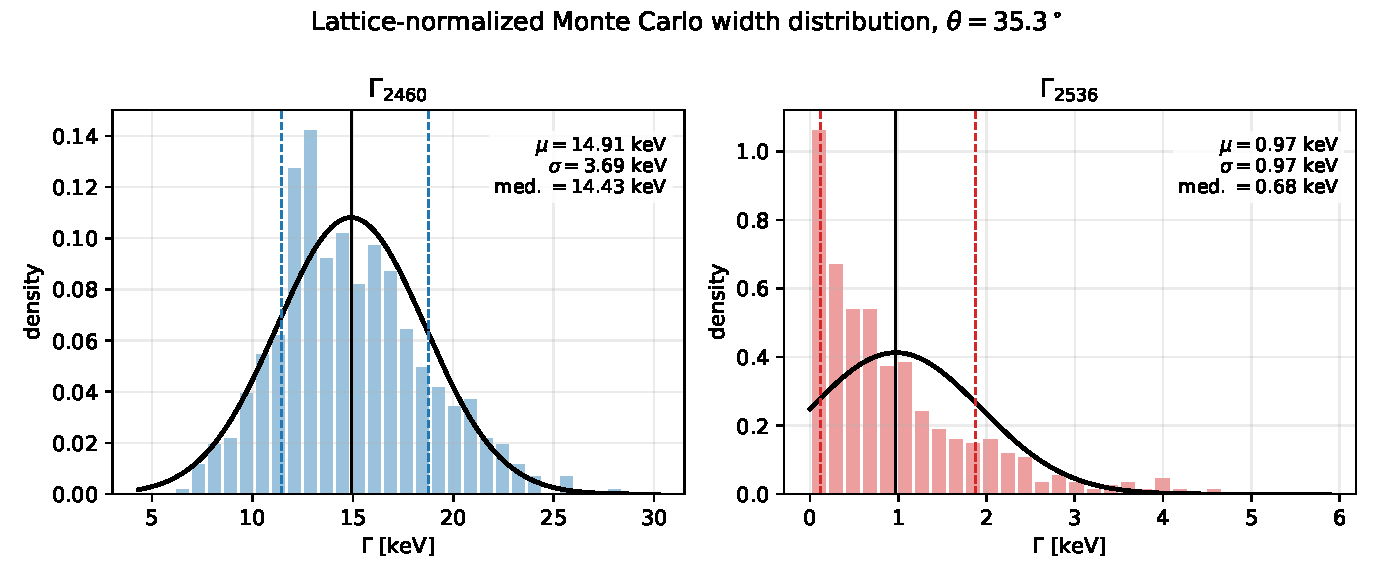
\includegraphics[width=0.47\textwidth]{../outputs/lattice_fperp_mc_width_histograms_theta_fixed.pdf}
  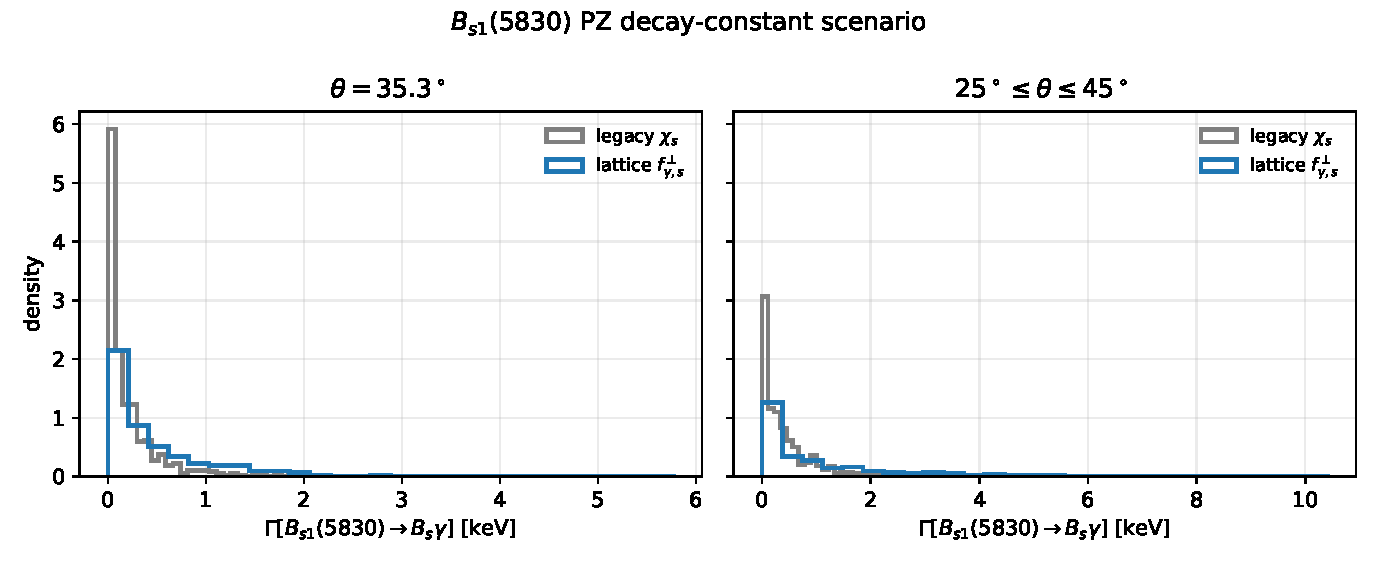
\includegraphics[width=0.47\textwidth]{../outputs/stage3_bs1_pz_width_histograms.pdf}
  \caption{Monte Carlo width distributions for the charm-strange lattice
  photon-normalization scenario (left) and the bottom-strange PZ
  decay-constant scenario (right).}
  \label{fig:mc-widths}
\end{figure}

\begin{figure}[htbp]
  \centering
  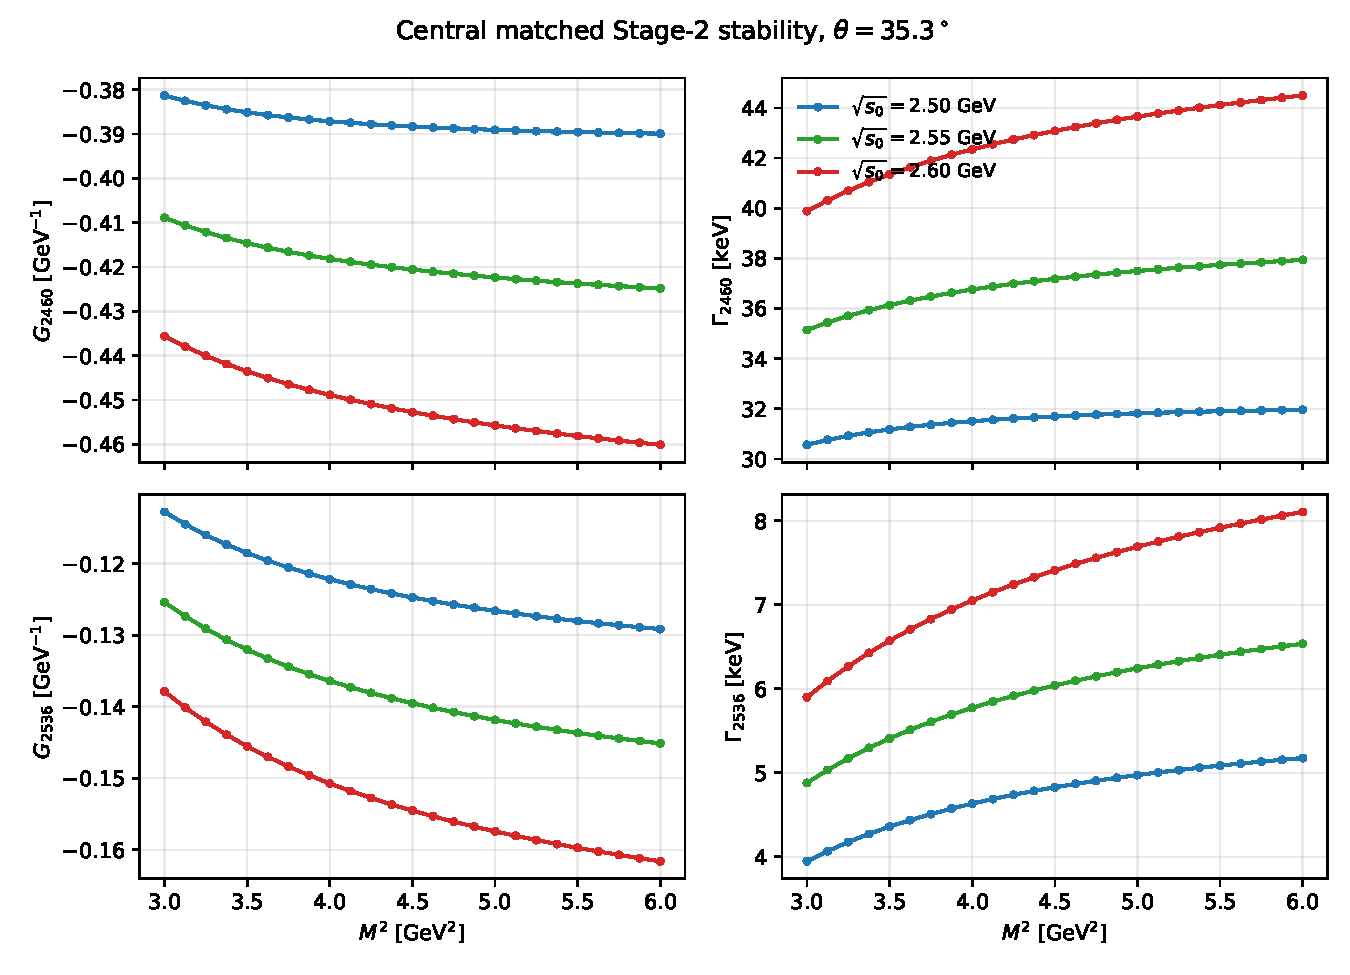
\includegraphics[width=0.47\textwidth]{../outputs/stage2_stability_central.pdf}
  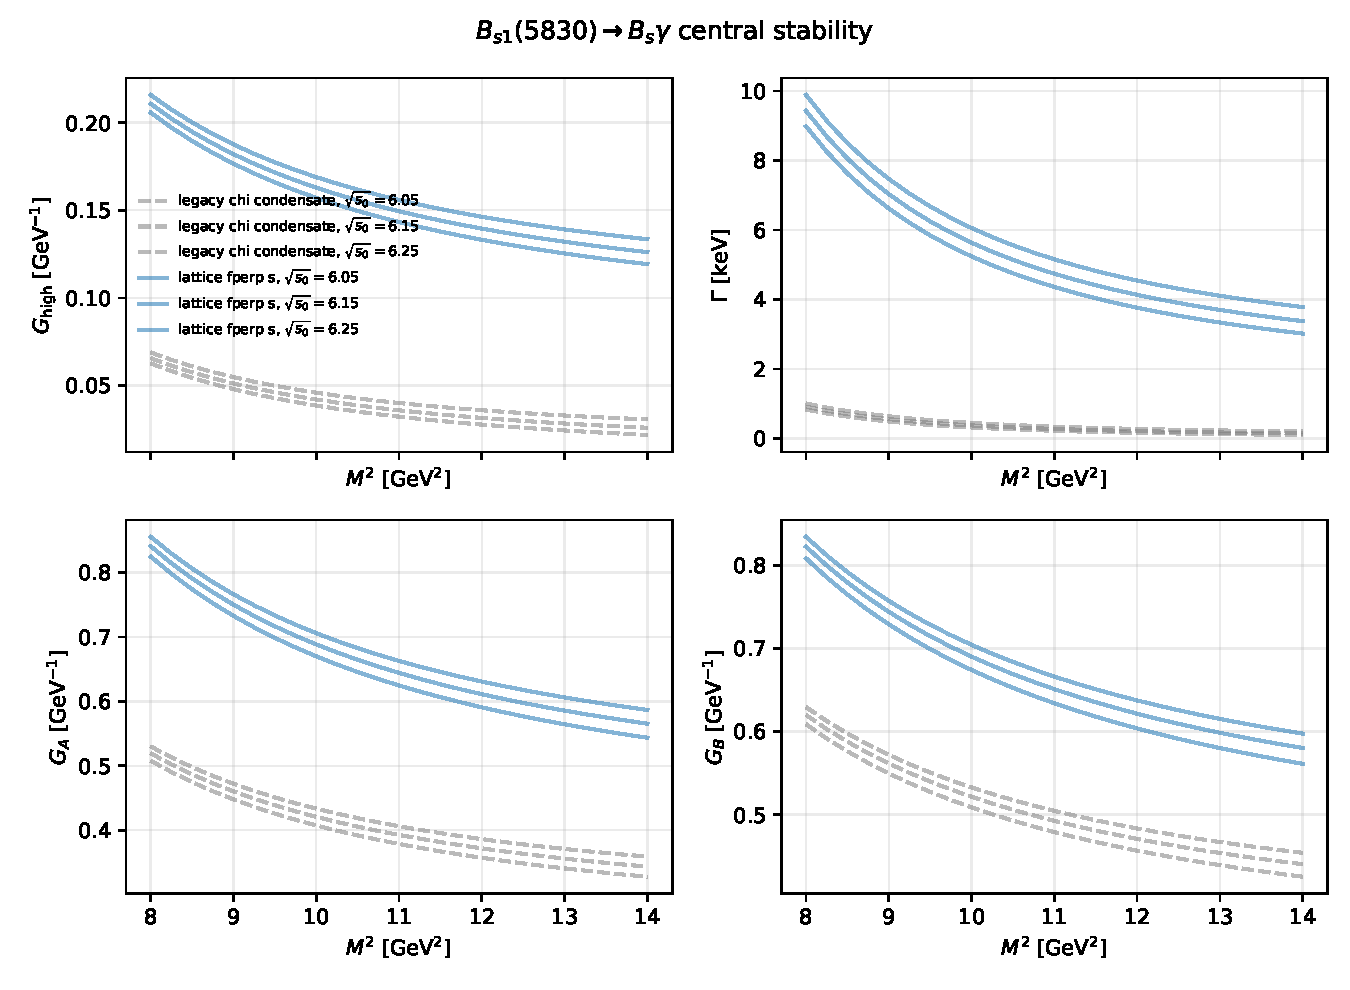
\includegraphics[width=0.47\textwidth]{../outputs/bs1_5830_stability.pdf}
  \caption{Representative stability plots in the selected Borel and continuum
  windows for the charm-strange and bottom-strange analyses.}
  \label{fig:stability}
\end{figure}

\section{Comparison with Experiment}

For $\Dsone(2460)$, BaBar measures a radiative branching fraction
$\mathcal B(\Dsone(2460)\to\Ds\gamma)=(16\pm4\pm3)\%$ \cite{BaBar2006}.  The
preferred lattice-normalized partial width,
$16.1^{+4.4}_{-3.7}~\keV$, corresponds to a total width of order
$0.10~\MeV$ if this branching fraction is used literally.  This is compatible
with the observed narrowness of the state.

For $\Dsone(2536)$, using the measured total width
$\Gamma_{\rm tot}=0.92\pm0.05~\MeV$ \cite{BaBar2011}, the preferred
lattice-normalized radiative width gives an estimated branching fraction of
order $5\times10^{-4}$.  The channel is therefore strongly cancellation
suppressed, which is consistent with the lack of a prominent experimental
signal.

For $\Bsone(5830)$, there is no direct radiative measurement.  Our PZ-normalized
prediction is a future-search target.  The median width remains below
$1~\keV$ in both photon-input scenarios, although the mixing-angle scan leaves
a long upper tail in the lattice-normalized case.

\section{Conclusions}

We have constructed a staged light-cone QCD sum-rule analysis of
$\Dsone\to\Ds\gamma$ and $\Bsone\to\Bs\gamma$ radiative transitions.  The
calculation includes hard photon emission from both quark lines, two-particle
photon DAs, three-particle photon DAs, and explicit strange-quark-mass terms.
The modern lattice normalization of the leading-twist photon DA reduces the
dominant photon-input ambiguity relative to the older susceptibility-only
scenario.  The resulting pattern is physically clear: $\Dsone(2460)$ can have a
visible radiative mode while $\Dsone(2536)$ and the observed high-combination
$\Bsone(5830)$ are cancellation suppressed.

\section*{Acknowledgments}

To be added.

\bibliographystyle{unsrt}
\bibliography{manuscript/references}

\end{document}
